\documentclass[english]{beamer}
\usetheme{default}
\usepackage{lmodern}
\usepackage[utf8]{inputenc}
\usepackage[T1]{fontenc}
\usepackage{babel}
\usepackage{color}
\usepackage{listings}
\usepackage{booktabs}
\usepackage{amsmath,amsthm,amssymb,graphicx,mathrsfs}
\usepackage{stmaryrd}
\usepackage{slashed}
%\usepackage[hmargin={3.5cm,3.5cm},top=4cm,bottom=4cm]{geometry} %problem...

\graphicspath{{images/}}

\newcommand{\cref}[1]{Eq.(\ref{#1})}
\newcommand{\ie}{\textit{i.e., }}
\newcommand{\eg}{\textit{e.g. }}
\newcommand{\wrt}{w.r.t. }
\newcommand{\rhs}{r.h.s. }
\newcommand{\lhs}{l.h.s. }
\newcommand{\eval}[1]{\bigg\rvert_{#1}}
\newcommand{\dd}{\textrm{d}}
%\newcommand{\de}{\textrm{e}}
\newcommand{\im}{\mathrm{Im}}
\newcommand{\ran}{\mathrm{Ran}}
\newcommand{\rank}{\mathrm{Rank}}
\newcommand{\dom}{\mathrm{Dom}}
\newcommand{\en}{\mathrm{End}}
\newcommand{\tr}{\mathrm{tr}}
\newcommand{\grad}{\mathrm{grad}}
\newcommand{\res}{\mathrm{Res}}
\newcommand{\Inf}{\mathrm{Inf}}
\newcommand{\dilog}{\mathrm{Li}_2}
\renewcommand{\thesection}{\arabic{section}} %to avoid the zero in front of the sections

\newcommand{\vb}[1]{\mathbf{#1}}
\newcommand{\V}[1]{\textnormal{#1}}
\newcommand{\bra}[1]{\langle#1 |}
\newcommand{\ket}[1]{| #1 \rangle}
\newcommand{\vdot}[0]{\boldsymbol\cdot}

\newtheorem{remark}{Remark}
\newtheorem{proposition}{Proposition}

\setbeamertemplate{footline}[frame number]{}
\setbeamertemplate{navigation symbols}{}
\setbeamertemplate{caption}[numbered]


%%%%%%%%%%%%%%%%%%%%%%%%%%%%
\lstset{%
  backgroundcolor=\color{white},   % choose the background color; you must add \usepackage{color} or \usepackage{xcolor}
  basicstyle=\small,        % the size of the fonts that are used for the code
  commentstyle=\color{blue},    % comment style
  extendedchars=true,              % lets you use non-ASCII characters; for 8-bits encodings only, does not work with UTF-8
  keepspaces=true,                 % keeps spaces in text, useful for keeping indentation of code (possibly needs columns=flexible)
  keywordstyle=\color{red},       % keyword style
  language=Fortran,                 % the language of the code
  rulecolor=\color{black},         % if not set, the frame-color may be changed on line-breaks within not-black text (e.g. comments (green here))
  showspaces=false,                % show spaces everywhere adding particular underscores; it overrides 'showstringspaces'
  showstringspaces=false,          % underline spaces within strings only
  showtabs=false,                  % show tabs within strings adding particular underscores
  stringstyle=\color{green},     % string literal style
  tabsize=2,                       % sets default tabsize to 2 spaces
  frame=single
}



%%%%%%%%%%%%%%%%%%%%%%%%%%%%%%%%%%%%%%%%%%%%%%%%%%%%%%%%%%%%%%%%%%%%%%%%
\title{Unitarity method in one-loop QCD amplitudes}
\author{En-Hung CHAO}
\institute{{\'E}cole Normale Sup{\'e}rieure}
\date{July 5th 2017}
%%%%%%%%%%%%%%%%%%%%%%%%%%%%%%%%%%%%%%%%%%%%%%%%%%%%%%%%%%%%%%%%%%%%%%%%
%%%%%%%%%%%%%%%%%%%%%%%%%%%%%%%%%%%%%%%%%%%%%%%%%%%%%%%%%%%%%%%%%%%%%%%%
\begin{document}
%\selectlanguage{english}
%\graphicspath{{../images/}}

\begin{frame}
\titlepage%
\centerline{supervised by David Kosower (IPhT, Saclay)}
\end{frame}
%%%%%%%%%%%%%%%%%%%%%%%%%%%%%%%%%%%%%%%
%%%%%%%%%%%%%%%%%%%%%%%%%%%%%%%%%
\begin{frame}
\frametitle{Outline}
\framesubtitle{}

\begin{enumerate}

\item Introduction
\item Spinor-helicity formalism
\item On-shell recursion
\item Generalized unitarity
\item Conclusion

\end{enumerate}

\end{frame}
%%%%%%%%%%%%%%%%%%%
\begin{frame}
\frametitle{Introduction}
\framesubtitle{}

\begin{itemize}
\item<1-> Motivation: perturbative computation at high energies in QCD \\ \eg high gluon multiplicity for jet, real gluon emission, loop-correction
\item<2-> Difficulties of traditional diagrammatic computation
    \begin{itemize}
    \item<3-> High graph multiplicity in non-abelian theories. \\ \eg beyond 4-gluon tree amplitude \tiny\color{blue}[Z. Bern, L. J. Dixon, D. C. Dunbar, \& D. A. Kosower, Nucl. Phys. B425 (1994)]\color{black}\normalsize
    \item<4-> Divergent loop integrals
    \end{itemize}
\item<5-> Solutions: use the analyticity and singularity structure of amplitudes
    \begin{itemize}
    \item<6-> Tree-level: on-shell recursion
    \item<7-> One-loop: generalized unitarity
    \end{itemize}
\item<8-> \textbf{Convention}: signature $(+,-,-,-)$, dimensional regularization in $D=4-2\epsilon$, massless particles
\end{itemize}
\end{frame}
%%%%%%%%%%%%%%%%%%
\begin{frame}[shrink=20]
\frametitle{Spinor-helicity formalism}
\framesubtitle{\tiny\color{blue}[L. J. Dixon, Proceedings, TASI-95]\color{black}\normalsize}
\begin{itemize}
\item<1-> 2-dimensional spinors from Dirac spinors in massless case
\begin{equation*}
\begin{split}
& v_+(p) = \begin{pmatrix}
|p]_\alpha \\ 0
\end{pmatrix} % := \lambda_p^\alpha
\quad,\quad
v_-(p) = \begin{pmatrix}
0 \\ |p\rangle^{\dot{\alpha}}
\end{pmatrix} % := \tilde{\lambda}_p^{\dot{\alpha}}
\\
& \bar{u}_-(p) = \begin{pmatrix} 
0, & \langle p |_{\dot{\alpha}}\end{pmatrix}
\quad,\quad
\bar{u}_+(p) = \begin{pmatrix} [ p|^\alpha, & 0 \end{pmatrix}
\end{split}
\end{equation*} 

\item<2-> Lorentz invariant products
\begin{equation*}
 \langle ij \rangle = \bar{u}_-(i)u_+(j) 
\quad,\quad
 [ij] = \bar{u}_+(i)u_-(j)
\end{equation*}

\item<3-> Momentum
\begin{equation*}
\slashed{p} = \begin{pmatrix}
0 & p_{a\dot{b}} \\ 
p^{\dot{a}b} & 0
\end{pmatrix} = |p\rangle [p| + |p]\langle p|
\quad,\quad
(p+q)^2 = \langle pq\rangle[qp]
\end{equation*}

\item<4-> Polarization vectors
\begin{equation*}
\varepsilon^+_\mu (p, q) = \frac{\langle q | \gamma_\mu |p]}{\sqrt{2}\langle qp \rangle}
\quad,\quad
\varepsilon^-_\mu (p, q) = -\frac{[q|\gamma_\mu | p\rangle}{\sqrt{2}[qp]}
\end{equation*}

\end{itemize}

\end{frame}
%%%%%%%%%%%%%%%%%%
\begin{frame}[shrink=30]
\frametitle{Spinor-helicity formalism}
\framesubtitle{}
\begin{itemize}
\item<1-> Color decomposition in a Yang-Mills theory
\\
\tiny\color{blue}[M. Mangano, Nucl. Phys. B 309
no. 3, (1988)][Z. Bern \& D. A. Kosower, Nucl. Phys. B 362 no. 1, (1991)]\color{black}\normalsize

\small
\begin{equation*}
\mathcal{A}_n^{\mathrm{tree}}(g_1, \ldots, g_n) = g'^{n-2}\sum_{\sigma\in\textrm{ permutation of }\{2,\ldots\}} A_n[1,\sigma(2),\ldots,\sigma(n))]\tr(T^{a_1} T^{a_{\sigma(2)}}\ldots T^{a_{\sigma(n)}})
\end{equation*}
\normalsize

$A_n[\ldots]$: color-ordered amplitude. 

\item<2-> Non-trivial 3-point all-gluon amplitudes
\begin{equation*}
A^{\mathrm{tree}}_3[g_1^- g_2^- g_3^+] = \frac{\langle 12 \rangle^3}{\langle 13 \rangle \langle 32 \rangle}
\quad,\quad
 A^{\mathrm{tree}}_3[g_1^+ g_2^+ g_3^-] = \frac{ [12]^3}{[13 ][ 32 ]}
\end{equation*}

\item<3-> Vanishing helicity configuration for $n\geq 4$
\begin{equation*}
A^{\mathrm{tree}}_n[g_1^\pm \ldots g_n^\pm] = A^{\mathrm{tree}}_n[g_1^\pm \ldots g_i^\mp \ldots g_n^\pm] = 0
\end{equation*}

\item<4-> First non-vanishing class: maximally-helicity-violating (MHV), given by the Parke-Taylor formulae
\tiny\color{blue}[S. J. Parke \& T. R. Taylor, Phys. Rev. Lett.
56 (1986)]
[F. Berends \& W. Giele, Nucl. Phys. B 306 no. 4, (1988)]
\color{black}\normalsize


\begin{equation*}
\begin{split}
& A^{\mathrm{tree}}_n[1^+\ldots i^-\ldots j^-\ldots n^+] = 
\frac{\langle ij \rangle^4}{\langle 12 \rangle\ldots \langle n1 \rangle}
\\
& A^{\mathrm{tree}}_n[1^-\ldots i^+\ldots j^+\ldots n^-] = 
\frac{[ ij]^4}{[ 12 ]\ldots [n1 ]}
\end{split}
\end{equation*}


\end{itemize}
\end{frame}
%%%%%%%%%%%%%%%%%%
\begin{frame}[shrink=20]
\frametitle{On-shell recursion}
\framesubtitle{
}
\begin{itemize}
\item<1-> Momentum shift
\\
\tiny\color{blue}
[R. Britto, F. Cachazo, \& B. Feng, Nucl. Phys. B 715 no. 1, (2005)] 
[R. Britto, F. Cachazo, B. Feng, \& E. Witten, Phys. Rev. Lett. 94
(2005)]
\color{black}\normalsize
\begin{equation*}
|\hat{i}] = |i] + z |j], \quad |\hat{j}] = |j], \quad|\hat{i}\rangle = |i\rangle, \quad |\hat{j}\rangle = |j\rangle - z|i\rangle
\end{equation*}  

\item<2-> Cauchy's theorem $\Rightarrow$ relation between shifted and unshifted amplitudes
\begin{equation*}
A_n = - \sum_{z = z_I}\res\frac{\hat{A}_n(z)}{z} + B_n
=\sum_{z = z_I} \hat{A}_L(z_I)\frac{1}{P_I^2}\hat{A}_R(z_I) + B_n
\end{equation*} 
\begin{figure}[h]
  \centering
  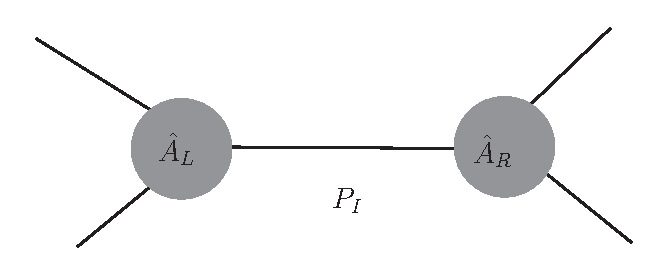
\includegraphics[width=0.5\linewidth]{bcfw.eps}
\end{figure}

\item<3-> $B_n$ vanishes under certain helicity configurations
\tiny\color{blue}[N. Arkani-Hamed \& J. Kaplan, JHEP 04 (2008)]
\color{black}\normalsize

\end{itemize}

\end{frame}
%%%%%%%%%%%%%%%%%%
\begin{frame}[shrink=30]
\frametitle{On-shell recursion}
\framesubtitle{Example: $A_6[1^-2^-3^-4^+5^+6^+]$}

\begin{itemize}
\item<1-> Possible configurations
\begin{figure}[h]
  \centering
  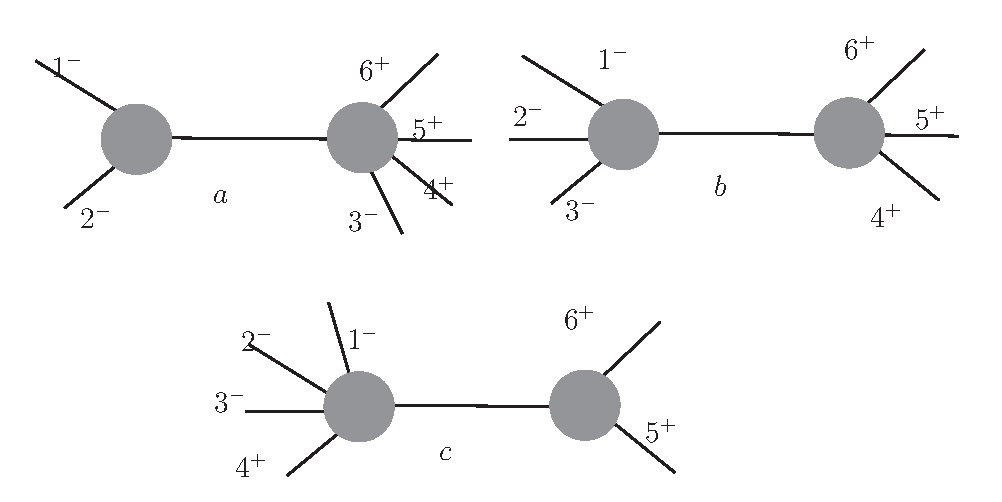
\includegraphics[width=0.8\linewidth]{A6nmhv.eps}
\end{figure}

\item[]<2->
\begin{equation*}
\begin{split}
A_6[1^-2^-3^-4^+5^+6^+] = & A_a + A_c 
\\ =&
-\frac{\langle 3 |\slashed{P}_{12}|6]^3}{[61]\langle 34\rangle \langle 45\rangle\langle 5|\slashed{P}_{16}|2][12]s_{126}}
-\frac{[4|\slashed{P}_{56}|1\rangle^3}{s_{156}\langle 5|\slashed{P}_{16}|2][23][34]\langle 56\rangle\langle 61\rangle}
\end{split}
\end{equation*} 

\end{itemize}

\end{frame}
%%%%%%%%%%%%%%%%%%
\begin{frame}[shrink=20]
\frametitle{Generalized unitarity}
\framesubtitle{}
\begin{itemize}
\item<1-> Master equation for one-loop
\begin{equation*}
A = \sum_i c_i I_i + \mathrm{rational} + \mathcal{O}(\epsilon)
\end{equation*}
\item<2-> Basis consists of master integrals
\\
\tiny\color{blue}
[J. Gluza, K. Kajda, \& D. A. Kosower, Phys. Rev. D83 (2011)
]
\color{black}\normalsize

\begin{figure}[h]
  \centering
  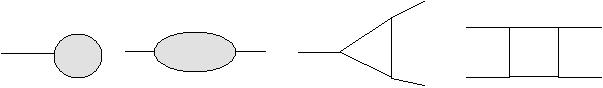
\includegraphics[width=0.5\linewidth]{master_integrals.jpg}
\end{figure}

\item<3-> Cutkosky rules and generalized unitarity
\tiny\color{blue}
[R. E. Cutkosky, Journal of Math. Phys. 1 no. 5, (1960)]
[Z. Bern, L. J. Dixon, D. C. Dunbar, and D. A. Kosower, Nucl. Phys. B425 (1994)]
\color{black}\normalsize
\begin{equation*}
\frac{1}{l^2 + i\epsilon} \rightarrow 2\pi i\delta^{(+)}\big(l^2\big)
\quad,\quad
\frac{1}{(l-K)^2 + i\epsilon} \rightarrow 2\pi i\delta^{(+)}\big((l-K)^2\big)
\end{equation*}
\small
\begin{equation*}
A(K^2 + i\epsilon) - A(K^2 - i\epsilon) =
-4\pi^2 \int\frac{\dd^D l}{(2\pi)^D}A^{\mathrm{tree}}_LA^{\mathrm{tree}}_R \delta^{(+)}(l^2)\delta^{(+)}\big((l-K)^2\big) 
\end{equation*}
\normalsize

\item<4-> Quadruple cut for box coefficients
    \tiny\color{blue}
[R. Britto, F. Cachazo, and B. Feng, Nucl. Phys. B725 (2005)]
\color{black}\normalsize
\begin{columns}
\begin{column}{0.5\textwidth}
\begin{figure}[h]
  \centering
  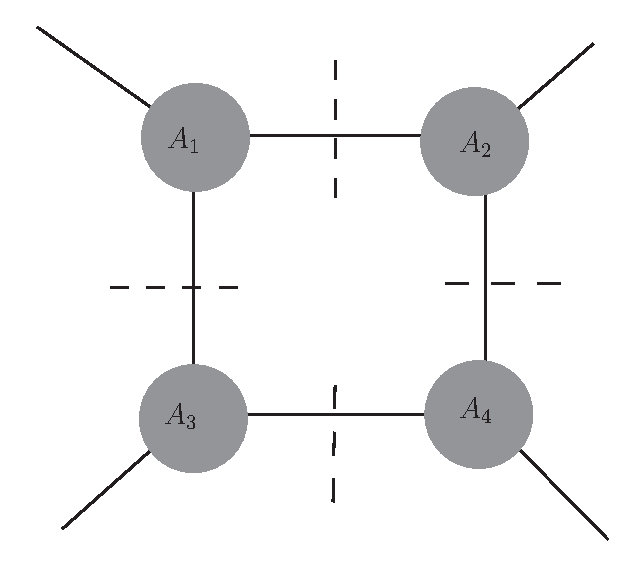
\includegraphics[width=0.4\linewidth]{quadruple_cut.eps}
\end{figure}\end{column}
\begin{column}{0.5\textwidth}  %%<--- here

\begin{equation*}
c = \frac{1}{2}\sum_{\mathcal{S}, J}n_J A_1^{\mathrm{tree}}A_2^{\mathrm{tree}}A_3^{\mathrm{tree}}A_4^{\mathrm{tree}}
\end{equation*}
\end{column}
\end{columns}


\end{itemize}

\end{frame}
%%%%%%%%%%%%%%%%%%
\begin{frame}[shrink=20]
\frametitle{Generalized unitarity}
\framesubtitle{}
\begin{itemize}
\item<1-> Triple cut for bubble and triangle coefficients
\tiny\color{blue}
[D. Forde, Phys. Rev. D75]
(2007)
\color{black}\normalsize
\begin{figure}[h]
  \centering
  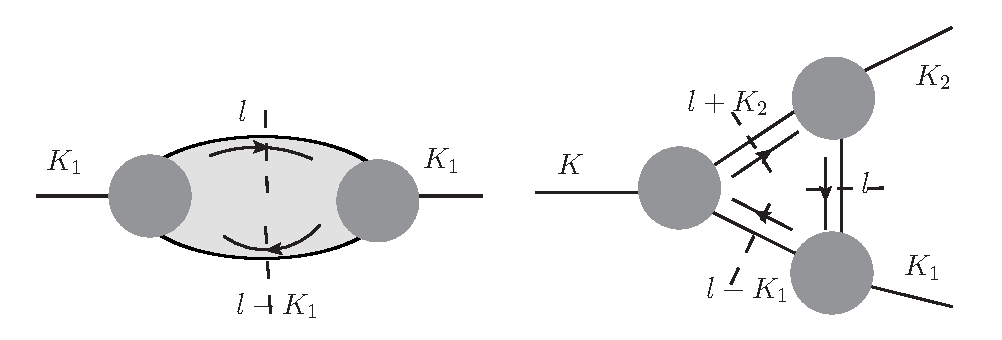
\includegraphics[width=0.7\linewidth]{triple_cut.eps}
\end{figure}

\item<2-> Parametrization of the loop momentum in a triple cut

\small
\begin{equation*}
l^\mu = \alpha_{02} K_1^{\flat,\mu} + \alpha_{01}K_2^{\flat,\mu} + \frac{t}{2}\langle K_1^\flat | \gamma^\mu |K_2^\flat] + \frac{\alpha_{01}\alpha_{02}}{2t}\langle K_2^\flat|\gamma^\mu |K_1^\flat]
\end{equation*}
\normalsize
where the two null vectors
\small
\begin{equation*}
K_1^\flat = K_1 - \frac{S_1}{\gamma}K_2^\flat \quad,\quad
K_2^\flat = K_2 - \frac{S_2}{\gamma}K_1^\flat
\end{equation*}
\normalsize
$\Rightarrow$ the triangle coefficient is given by the $t^0$ term of $\mathrm{Inf}_t(A_1A_2A_3)(t)$

\item<3-> Parametrization for bubble with a null vector $\chi$
\small
\begin{equation*}
l^\mu = yK_1^{\flat,\mu} + \frac{S_1}{\gamma}(1-y)\chi^\mu + \frac{t}{2}\langle K_1^\flat|\gamma^\mu|\chi] + \frac{S_1}{2\gamma}\frac{y}{t}(1-y)\langle \chi|\gamma^\mu|K_1^\flat]
\end{equation*}
\normalsize
\item<4->[]
The coefficient is determined with a double and a triple cut
\begin{equation*}
b = -i[\Inf_t[\Inf_y A_1 A_2](y)](t)\big|_{t\rightarrow 0 , y^m\rightarrow \frac{1}{m+1}}
-\frac{1}{2}\sum_{C_{\mathrm{tri}}}[\Inf_t A_1A_2A_3](t)\big|_{t^j\rightarrow T(j)}
\end{equation*} 

\end{itemize}

\end{frame}
%%%%%%%%%%%%%%%%%%
\begin{frame}[shrink=20]
\frametitle{Generalized unitarity}
\framesubtitle{}
\begin{itemize}
\item<1-> Cut-constructibility: branch cuts come from the (poly-)logarithms
\tiny
\begin{equation*}
\begin{split}
I^{\mathrm{2me}}_4 = &\frac{2i\Gamma(1+\epsilon)}{(4\pi)^{2-\epsilon}}\frac{ \Gamma^2(1-\epsilon)}{\Gamma(1-2\epsilon)}\frac{1}{st-K_1^2K_3^2}\frac{1}{\epsilon^2}
\Big[
(-s)^{-\epsilon} - (-K_1^2)^{-\epsilon} - (-K_3^2)^{-\epsilon} + (-t)^{-\epsilon}
\\&
+\epsilon^2\Big(
\dilog\big(1-\frac{K_1^2K_3^2}{st}\big) 
-\dilog\big(1-\frac{K_1^2}{s}\big) 
-\dilog\big(1-\frac{K_1^2}{t}\big) 
-\dilog\big(1-\frac{K_3^2}{s}\big) 
-\dilog\big(1-\frac{K_3^2}{t}\big) 
-\frac{1}{2}\ln^2\big(\frac{s}{t}\big)
\Big)
\Big]
+\mathcal{O}(\epsilon)
\end{split}
\end{equation*}
\normalsize
\item<2->[]
$\Rightarrow$ ambiguity: polynomial terms in kinematic invariants do not contribute to branch cut

\item<3-> Decomposition of a $D=4-2\epsilon$ dimensional loop-momentum and the integration measure

\begin{equation*}
l^\nu = \bar{l}^\nu + l_{[-2\epsilon]}^\nu = \bar{l}^2 - \mu^2
\quad,\quad
\int\frac{\dd^D l}{(2\pi)^D} = 
\int\frac{\dd^{-2\epsilon}(\mu^2)}{(2\pi)^{-2\epsilon}}\int\frac{\dd^4 \bar{l}}{(2\pi)^4}
\end{equation*}

\item<4-> The rational term can be determined from the singularity structure using similar parametrizations as before
\tiny\color{blue}
[S. D. Badger, JHEP 01 (2009)]
\color{black}\small
\begin{equation*}
\begin{split}
& R_n = -\frac{1}{6}\sum_{K_4}C_{4,K_4}^{[4]} - \frac{1}{2}\sum_{K_3}C_{3,K_3}^{[2]} - 
\frac{1}{6}\sum_{K_2}\big(K_2^2 - 3(m_1^2 + m_2^2)\big)C_{2,K_2}^{[2]}
\\
& C_4^{[4]} = \frac{i}{2}\sum_{\sigma}\Inf_{\mu^2}[A_1A_2A_3A_4(\bar{l}^\sigma)]\big|_{\mu^4}
\\
& C_3^{[2]} = \frac{1}{2}\sum_\sigma\Inf_{\mu^2}[\Inf_t[A_1A_2A_3(\bar{l}^\sigma)]\big|_{t^0}]\big|{\mu^2}
\\
& C_2^{[2]} = -i\Inf_{\mu^2}[\Inf_t[\Inf_y A_1 A_2(\bar{l}(y,t,\mu^2))]]]\big|_{\mu^2,t^0,y^i\rightarrow Y_i} -\frac{1}{2}\sum_{\sigma}\Inf_{\mu^2}[\Inf_tA_1A_2A_3^{K_3}(\bar{l}, t, \mu^2)]]\big|_{\mu^2,t^i\rightarrow T_i}
\end{split}
\end{equation*}

\end{itemize}

\end{frame}
%%%%%%%%%%%%%%%%%%
\begin{frame}
\frametitle{Summary}
\framesubtitle{}
\begin{itemize}
\item<1-> Spinor-helicty formalism provides a compact way of writing amplitudes
\item<2-> The on-shell recursion uses the analyticity of amplitudes and avoids computing Feynman diagrams individually
\item<3-> Generalized unitarity allows to construct one-loop amplitudes from tree-level ones

\end{itemize}

\end{frame}


\end{document}

















